\documentclass[color=usenames,dvipsnames]{beamer}\usepackage[]{graphicx}\usepackage[]{color}
% maxwidth is the original width if it is less than linewidth
% otherwise use linewidth (to make sure the graphics do not exceed the margin)
\makeatletter
\def\maxwidth{ %
  \ifdim\Gin@nat@width>\linewidth
    \linewidth
  \else
    \Gin@nat@width
  \fi
}
\makeatother

\definecolor{fgcolor}{rgb}{0, 0, 0}
\newcommand{\hlnum}[1]{\textcolor[rgb]{0.69,0.494,0}{#1}}%
\newcommand{\hlstr}[1]{\textcolor[rgb]{0.749,0.012,0.012}{#1}}%
\newcommand{\hlcom}[1]{\textcolor[rgb]{0.514,0.506,0.514}{\textit{#1}}}%
\newcommand{\hlopt}[1]{\textcolor[rgb]{0,0,0}{#1}}%
\newcommand{\hlstd}[1]{\textcolor[rgb]{0,0,0}{#1}}%
\newcommand{\hlkwa}[1]{\textcolor[rgb]{0,0,0}{\textbf{#1}}}%
\newcommand{\hlkwb}[1]{\textcolor[rgb]{0,0.341,0.682}{#1}}%
\newcommand{\hlkwc}[1]{\textcolor[rgb]{0,0,0}{\textbf{#1}}}%
\newcommand{\hlkwd}[1]{\textcolor[rgb]{0.004,0.004,0.506}{#1}}%
\let\hlipl\hlkwb

\usepackage{framed}
\makeatletter
\newenvironment{kframe}{%
 \def\at@end@of@kframe{}%
 \ifinner\ifhmode%
  \def\at@end@of@kframe{\end{minipage}}%
  \begin{minipage}{\columnwidth}%
 \fi\fi%
 \def\FrameCommand##1{\hskip\@totalleftmargin \hskip-\fboxsep
 \colorbox{shadecolor}{##1}\hskip-\fboxsep
     % There is no \\@totalrightmargin, so:
     \hskip-\linewidth \hskip-\@totalleftmargin \hskip\columnwidth}%
 \MakeFramed {\advance\hsize-\width
   \@totalleftmargin\z@ \linewidth\hsize
   \@setminipage}}%
 {\par\unskip\endMakeFramed%
 \at@end@of@kframe}
\makeatother

\definecolor{shadecolor}{rgb}{.97, .97, .97}
\definecolor{messagecolor}{rgb}{0, 0, 0}
\definecolor{warningcolor}{rgb}{1, 0, 1}
\definecolor{errorcolor}{rgb}{1, 0, 0}
\newenvironment{knitrout}{}{} % an empty environment to be redefined in TeX

\usepackage{alltt}
%\documentclass[color=usenames,dvipsnames,handout]{beamer}

\usepackage[sans]{../lab1}
\usepackage[hang,flushmargin]{footmisc}
\usepackage{tikz}
\usetikzlibrary{shapes,arrows,snakes,backgrounds}


\hypersetup{pdftex,pdfstartview=FitV}






%% New command for inline code that isn't to be evaluated
\definecolor{inlinecolor}{rgb}{0.878, 0.918, 0.933}
\newcommand{\inr}[1]{\colorbox{inlinecolor}{\texttt{#1}}}


\title[slides]{Some thoughts on experimental design and
  graduate student research}
\author{Richard Chandler \\ Based on presentation by Dr. Bob Cooper}
\date{September 9, 2021}
\IfFileExists{upquote.sty}{\usepackage{upquote}}{}
\begin{document}


\begin{frame}[plain]
  % \maketitle
  \centering
  \LARGE
  Some Thoughts on Experimental Design and Graduate Student Research \\
  \vfill
  \large
  Richard Chandler \\
  (Based on presentation by Dr. Bob Cooper) \\
  Warnell School of Forestry and Natural Resources \\
  September 9, 2021
\end{frame}



\begin{frame}
  \frametitle{Outline}
  \Large
  \tableofcontents%[hideallsubsections]}
\end{frame}


\section{Background}


\begin{frame}
  \frametitle{Science}
  The purpose of scientific research is to advance knowledge. \\
  \pause
  \vfill
  We want to understand causal relationships between variables. \\
  \begin{itemize}
    \item How does drug $X$ affect disease $Y$?
    \item How does management practice $X$ affect species $Y$?
  \end{itemize}
  \pause
  \vfill
  Two general approaches for achieving causal inference:
  \begin{itemize}
    \item Manipulative experiments
    \item Observational studies (usually considered inferior)
  \end{itemize}
\end{frame}



% \begin{frame}
%   \frametitle{The Scientific Method}
%   \begin{enumerate}[1.]
%     \item State the problem
%     \item Formulate the hypothesis
%     \item Design the experiment or observational study
%     \item Make observations
%     \item Analyze data
%     \item Draw conclusions
%     \end{enumerate}
% \vfill    
% \centering    
% Where does statistical analysis fit in?  Where do most courses in
% statistics apply to the scientific method? \\
% \vfill
% Where does experimental design fit in?  Courses? \\
% \end{frame}



\begin{frame}
  \frametitle{Terminology for experiments}
  \small
  {\bf Experiment} \\
  An act or operation for the purpose of discovering something
  unknown. \par
  \pause
  \vfill %\vspace{12pt}
  {\bf Experimental unit} \\
  The unit to which the treatments are applied. \par
  % \vfill
  \pause
  \vfill %\vspace{12pt}
  {\bf Manipulative experiment} \\
  An experiment in which the experimental units receive different
  treatments and the assignment of treatments is or can be randomized. \\
  % \vfill
  % \pause
  % \vspace{12pt}
  % {\bf Observational study} \\
  % Research that involves only the making of measurements at one
  % or more points in space or time (a.k.a. mesurative experiment). \par
%  \vfill
  % \vspace{2pt}
  % \rule[0mm]{1cm}{0.1mm} \\
  % \footnotesize
  % Hurlbert, S.A. (1984) Pseudoreplication and the design of ecological field
  % experiments.  Ecological Monographs 54:187-211.
  \pause
  \vfill
  {\bf Response variable } \\
  The variable that is the focus of the research. Also known as the
  dependent variable or outcome variable.
  \pause
  \vfill
  {\bf Treatment variable } \\
  A variable thought to affect the response variable. Also known as the 
  explanatory variable, independent variable, or predictor variable.
\end{frame}




\begin{frame}
  \frametitle{Terminology}
  {\bf Experimental Design:} %\\
  The logical structure of an experiment. \\ %(Fisher 1971) \\
  \vspace{6pt}
  \vfill  
  Includes:
  \begin{itemize}
    \item Type of experimental units employed
    \item Number of treatment types (including controls)
    \item Response variables measured
    \item Manner in which treatments are applied
    \item Number of experimental units receiving each treatment (replicates)
    \item Physical and temporal arrangement of experimental units
    \item Controlling extraneous sources of variability, etc.
  \end{itemize}
  \vfill
  \vspace{6pt}
  \rule[0mm]{1cm}{0.1mm} \\
  \footnotesize
  Fisher, R.A. (1971) The Design of Experiments. Macmillan. 
\end{frame}




\section{Experiments}


\begin{frame}
  \frametitle{Features of good experimental design}
  \pause
  \small
  {\bf Replication} \\
  More than one experimental unit or replicate per treatment. \\
  Allows one to account for variability among experimental units and
  obtain precise parameter estimates. \\
  \pause
  \vfill
  {\bf Randomization} \\
  All units must have pre-determined probabilities of receiving each
  treatments. Otherwise, estimates may be biased. \\
  \pause
  \vfill
  {\bf Controls} \\
  Allow one to isolate the causative agent of interest (treatment
  effect). \\ % Not always an untreated treatment. \\
  \pause
  \vfill
  {\bf Interspersion} \\
  Hurlbert's (1984) recommendation that treatments be spatially interspersed.  \\
  \vspace{1pt}
  \rule[0mm]{1cm}{0.1mm} \\
  \footnotesize
  Hurlbert, S.A. (1984) Pseudoreplication and the design of ecological field
  experiments.  Ecological Monographs 54:187-211.
\end{frame}



\begin{frame}
  \frametitle{Example: Timber harvest and salamanders}
  Suppose we wish to assess the effect of timber harvest on salamander
  abundance.  One plot is established in each of two forests, one
  thinned and the other untreated, in which we trap salamanders at $n=9$
  pitfall traps.  %The response variable of interest is the number of a
  %species captured per trap.  The explanatory variable is silvicultural
  %treatment. \\
  \vfill
  \centering
  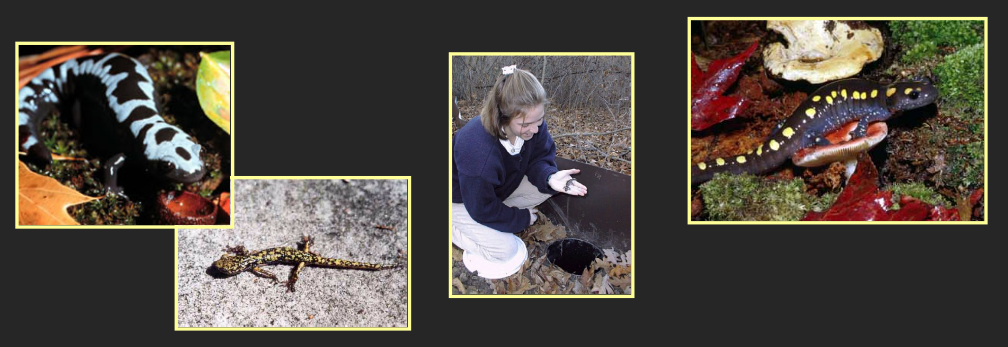
\includegraphics[width=\textwidth]{salamanders} \\
\end{frame}


\begin{frame}
  \frametitle{Example: Timber harvest and salamanders}
  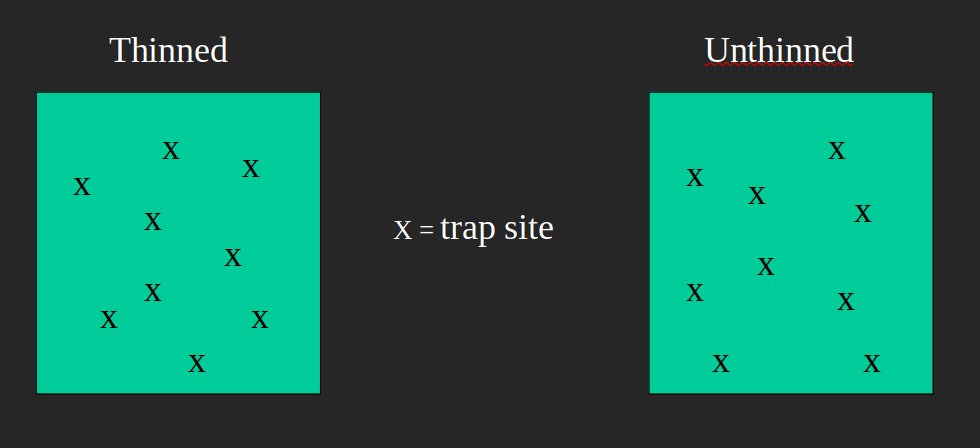
\includegraphics[width=\textwidth]{salamander-design} \\
  \vfill
  The response variable of interest is the number of red-backed
  salamanders captured per trap.  The explanatory variable is harvest
  treatment (thinned/not). We find more salamanders on the untreated
  plot, and conclude that thinning is bad for salamanders.  What is
  wrong with this design?  
\end{frame}


\begin{frame}
  \frametitle{Example: Timber harvest and salamanders}
  {\bf Problems}
  \begin{itemize}
    \item Unreplicated
      \begin{itemize}
      \item Impossible to account for other sources of variation.
      \item Increasing sample size will yield more precise estimates
        of treatment effects.
        \end{itemize}
    \item[]
    \item<2-> No randomization
      \begin{itemize}
        \item Confounding of sources of variation -- is the difference
          due to treatment or location or some other unmeasured variable? 
        \item Randomization will reduce potential for bias in
          estimates of treatment effects.
      \end{itemize}      
    \item[]
    \item<3-> Pseudoreplication
      \begin{itemize}
      \item Incorrect error degrees of freedom in a statistical test.
      \end{itemize}
    \end{itemize}
\end{frame}


\begin{frame}[fragile]
  \frametitle{Replication}
  Without replication {\it of experimental units}, we don't know if
  differences are due to other sources of variation. \\
  % R code
  \vfill
\begin{knitrout}\scriptsize
\definecolor{shadecolor}{rgb}{0.878, 0.918, 0.933}\color{fgcolor}

{\centering \includegraphics[width=0.75\textwidth]{figure/replication-1} 

}


\end{knitrout}
\end{frame}




\begin{frame}[fragile]
  \frametitle{Replication}
  Here's what happens with $n=1$ experimental unit (per treatment) \\
\begin{knitrout}\scriptsize
\definecolor{shadecolor}{rgb}{0.878, 0.918, 0.933}\color{fgcolor}\begin{kframe}
\begin{alltt}
\hlstd{meanAbundanceThinned} \hlkwb{<-} \hlnum{10}      \hlcom{## Mean salamanders in thinned}
\hlstd{meanAbundanceUnthinned} \hlkwb{<-} \hlnum{15}    \hlcom{## Mean salamanders in unthinned}
\hlstd{StdDev} \hlkwb{<-} \hlnum{3}                     \hlcom{## Variability among experimental units}
\hlstd{dataThinned} \hlkwb{<-} \hlkwd{rnorm}\hlstd{(}\hlkwc{n}\hlstd{=}\hlnum{1}\hlstd{, meanAbundanceThinned, StdDev)}
\hlstd{dataUnthinned} \hlkwb{<-} \hlkwd{rnorm}\hlstd{(}\hlkwc{n}\hlstd{=}\hlnum{1}\hlstd{, meanAbundanceUnthinned, StdDev)}
\hlkwd{t.test}\hlstd{(dataThinned, dataUnthinned,} \hlkwc{var.equal}\hlstd{=}\hlnum{TRUE}\hlstd{)}
\end{alltt}


{\ttfamily\noindent\bfseries\color{errorcolor}{\#\# Error in t.test.default(dataThinned, dataUnthinned, var.equal = TRUE): not enough observations}}\end{kframe}
\end{knitrout}
\end{frame}




\begin{frame}[fragile]
  \frametitle{Replication}
  Things look better with $n=10$ experimental units \\
\begin{knitrout}\scriptsize
\definecolor{shadecolor}{rgb}{0.878, 0.918, 0.933}\color{fgcolor}\begin{kframe}
\begin{alltt}
\hlstd{dataThinned} \hlkwb{<-} \hlkwd{rnorm}\hlstd{(}\hlkwc{n}\hlstd{=}\hlnum{10}\hlstd{, meanAbundanceThinned, StdDev)}
\hlstd{dataUnthinned} \hlkwb{<-} \hlkwd{rnorm}\hlstd{(}\hlkwc{n}\hlstd{=}\hlnum{10}\hlstd{, meanAbundanceUnthinned, StdDev)}
\hlkwd{t.test}\hlstd{(dataThinned, dataUnthinned,} \hlkwc{var.equal}\hlstd{=}\hlnum{TRUE}\hlstd{)}
\end{alltt}
\begin{verbatim}
## 
## 	Two Sample t-test
## 
## data:  dataThinned and dataUnthinned
## t = -3.9452, df = 18, p-value = 0.0009489
## alternative hypothesis: true difference in means is not equal to 0
## 95 percent confidence interval:
##  -9.821058 -2.995730
## sample estimates:
## mean of x mean of y 
##  8.725764 15.134158
\end{verbatim}
\end{kframe}
\end{knitrout}
\end{frame}



\begin{frame}
  \frametitle{Randomization}
  \small
  Without randomization, the observed effect could be due to a
  \alert{confounding variable}. For example, imagine that thinning
  does not influence salamander abundance, but \alert{distance to
    stream} is a {\it common cause} of both thinning and salamander
  abundance. \\  
  \vfill
  \begin{center}
    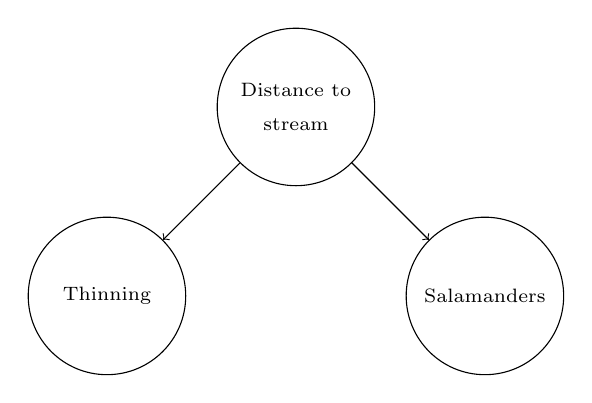
\begin{tikzpicture}[scale=0.8]
      \node[circle,draw,minimum size=2cm] at (0,0) (x1) {\scriptsize Thinning}; 
      \node[circle,draw,minimum size=2cm,align=center] at (3,3) (x2)
        {\scriptsize Distance to \\ \scriptsize stream}; 
      \node[circle,draw,minimum size=2cm] at (6,0) (y) {\scriptsize Salamanders}; 
%      \draw[->] (x1) to (y);
      \draw[->] (x2) to (y);
      \draw[->] (x2) to (x1);
   \end{tikzpicture}
 \end{center}
 \pause
 \vfill
 If we select treatment plots based on distance to stream, we might
 find a spurious effect of thinning, even though thinning has no
 causal effect.  
\end{frame}


%\begin{frame}[fragile]
%  \frametitle{Randomization}

%\end{frame}



\begin{frame}
  \frametitle{Experimental Designs}
  \centering
  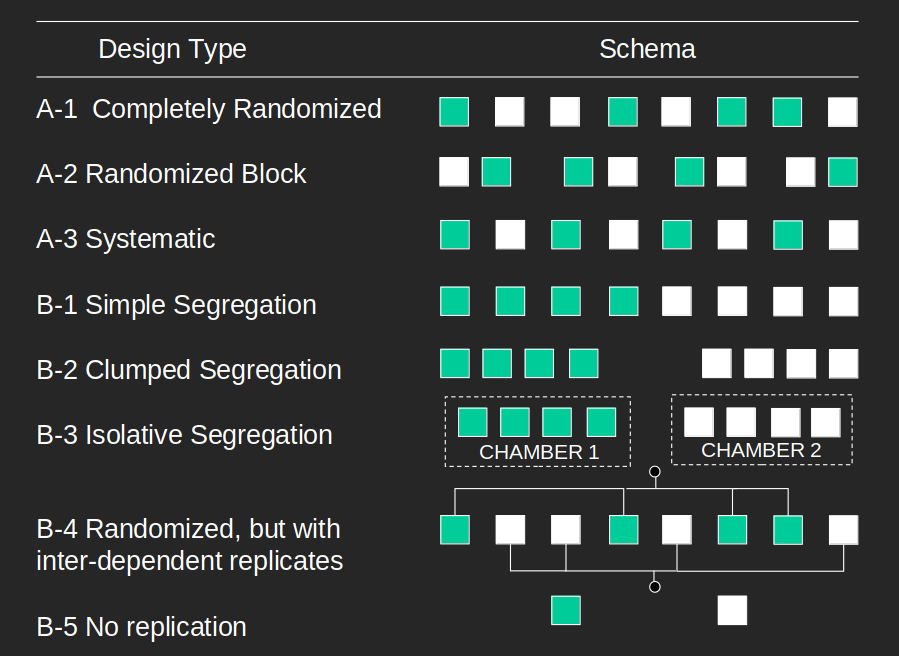
\includegraphics[width=0.8\textwidth]{Hurlbert-schema} \\
  \vfill
  Fig. 1 from Hurlbert (1984). Good designs (A) and designs without
  interspersion (B). \\
\end{frame}



\section{Observational Studies}



\begin{frame}
  \frametitle{Outline}
  \Large
  \tableofcontents[currentsection]
\end{frame}



\begin{frame}
  \frametitle{Example 2: Growth and survival of
    tree seedlings in a bottomland forest}
  Suppose we wish to understand the factors that influence growth and
  survival of tree seedlings in a periodically flooded bottomland
  forest.  Depending on our objectives (and prior knowledge), we might
  take several approaches to address this topic. \\
  \vfill
  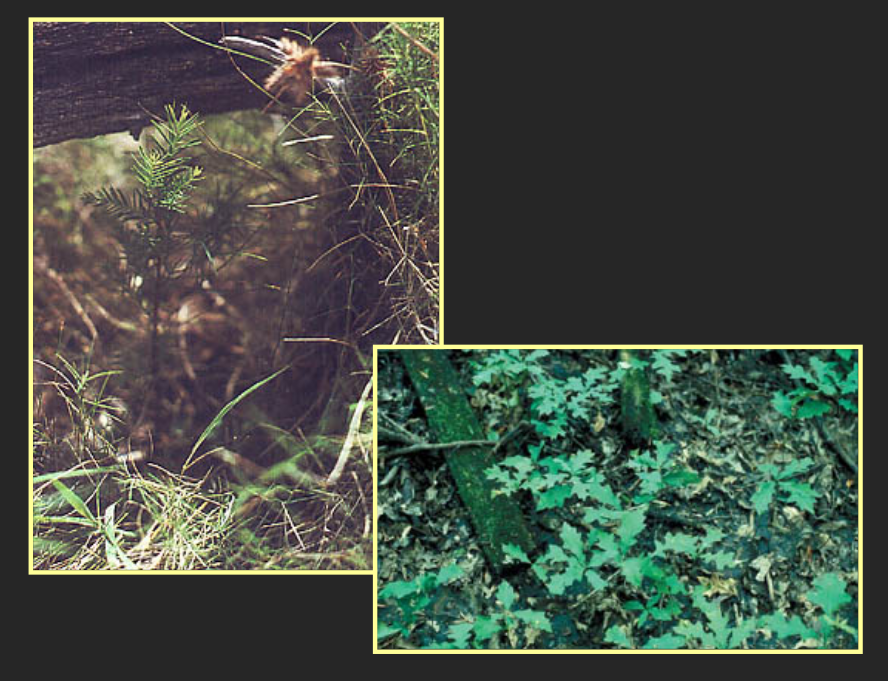
\includegraphics[height=1.6in]{seedlings-obs} \hfill
  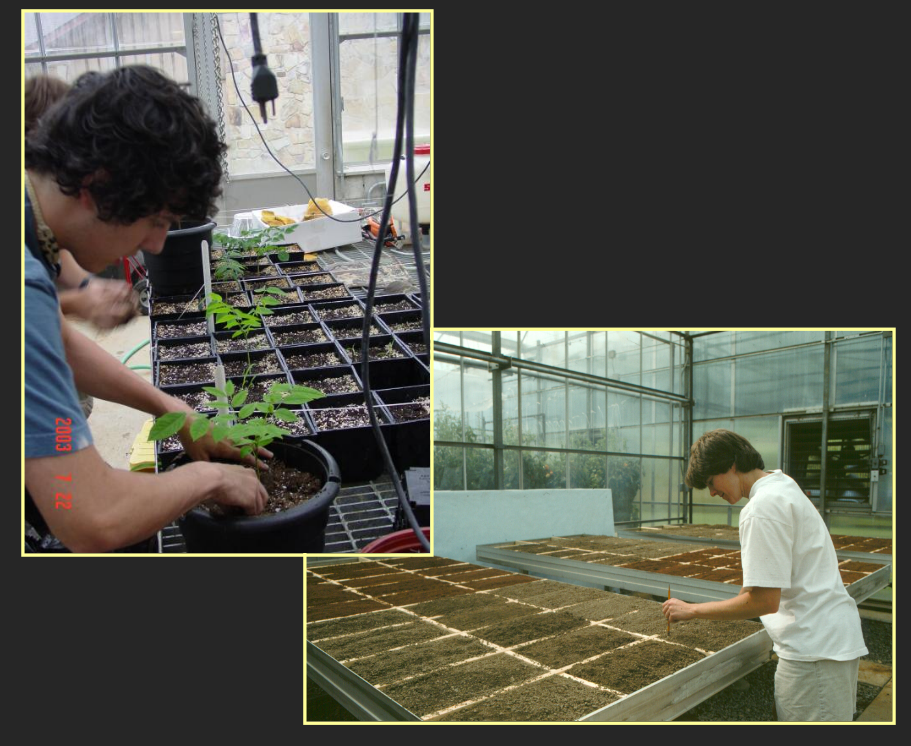
\includegraphics[height=1.6in]{seedlings-exp} 
\end{frame}



\begin{frame}
  \frametitle{Example 2: Growth and survival of
    tree seedlings in a bottomland forest}
  Option 1: Manipulative experiment -- focus on a few key variables of
  particular interest and attempt to hold all else constant.
  \vspace{6pt}
  \begin{itemize}
    \item For example, manipulate shading and flooding (plus
      interactions) in a greenhouse setting.
    \item Other factors (soil, herbivory, etc.)  held constant.
    \item Features of good experimental design still needed, even in a
      highly controlled laboratory and greenhouse setting.
    \item Cause and effect can be established in the greenhouse, but
      will they extrapolate to a field setting?
  \end{itemize}
\end{frame}



\begin{frame}
  \frametitle{Example 2: Growth and survival of
    tree seedlings in a bottomland forest}
  Option 2: Observation study -- measure factors (variables) {\it in
    situ} that you think will influence growth and survival of seedlings. 
  \vspace{6pt}
  \begin{itemize}
    \item Control and manipulate nothing
    \item Examine correlations between growth of seedlings and
      the explanatory variables
    \item Find the best model from a candidate set based upon
      hypotheses. Models should be predictive and
      mechanistic (based on theory).
    \item Must be wary of confounding variables, especially
      confounders that cannot (or were not) be measured.
    \item Remember that {\it ``correlation does not imply
        causation''}, but in certain cases it does. 
  \end{itemize}
\end{frame}



\begin{frame}
  \frametitle{Causal inference in observational studies}
  \small
  A huge body of literature now exists on causal inference in
  observational studies. These methods allow researchers to determine
  when causal effects can be estimated without manipulation. Details
  are fairly technical. \\ 
  \vfill
  \centering
  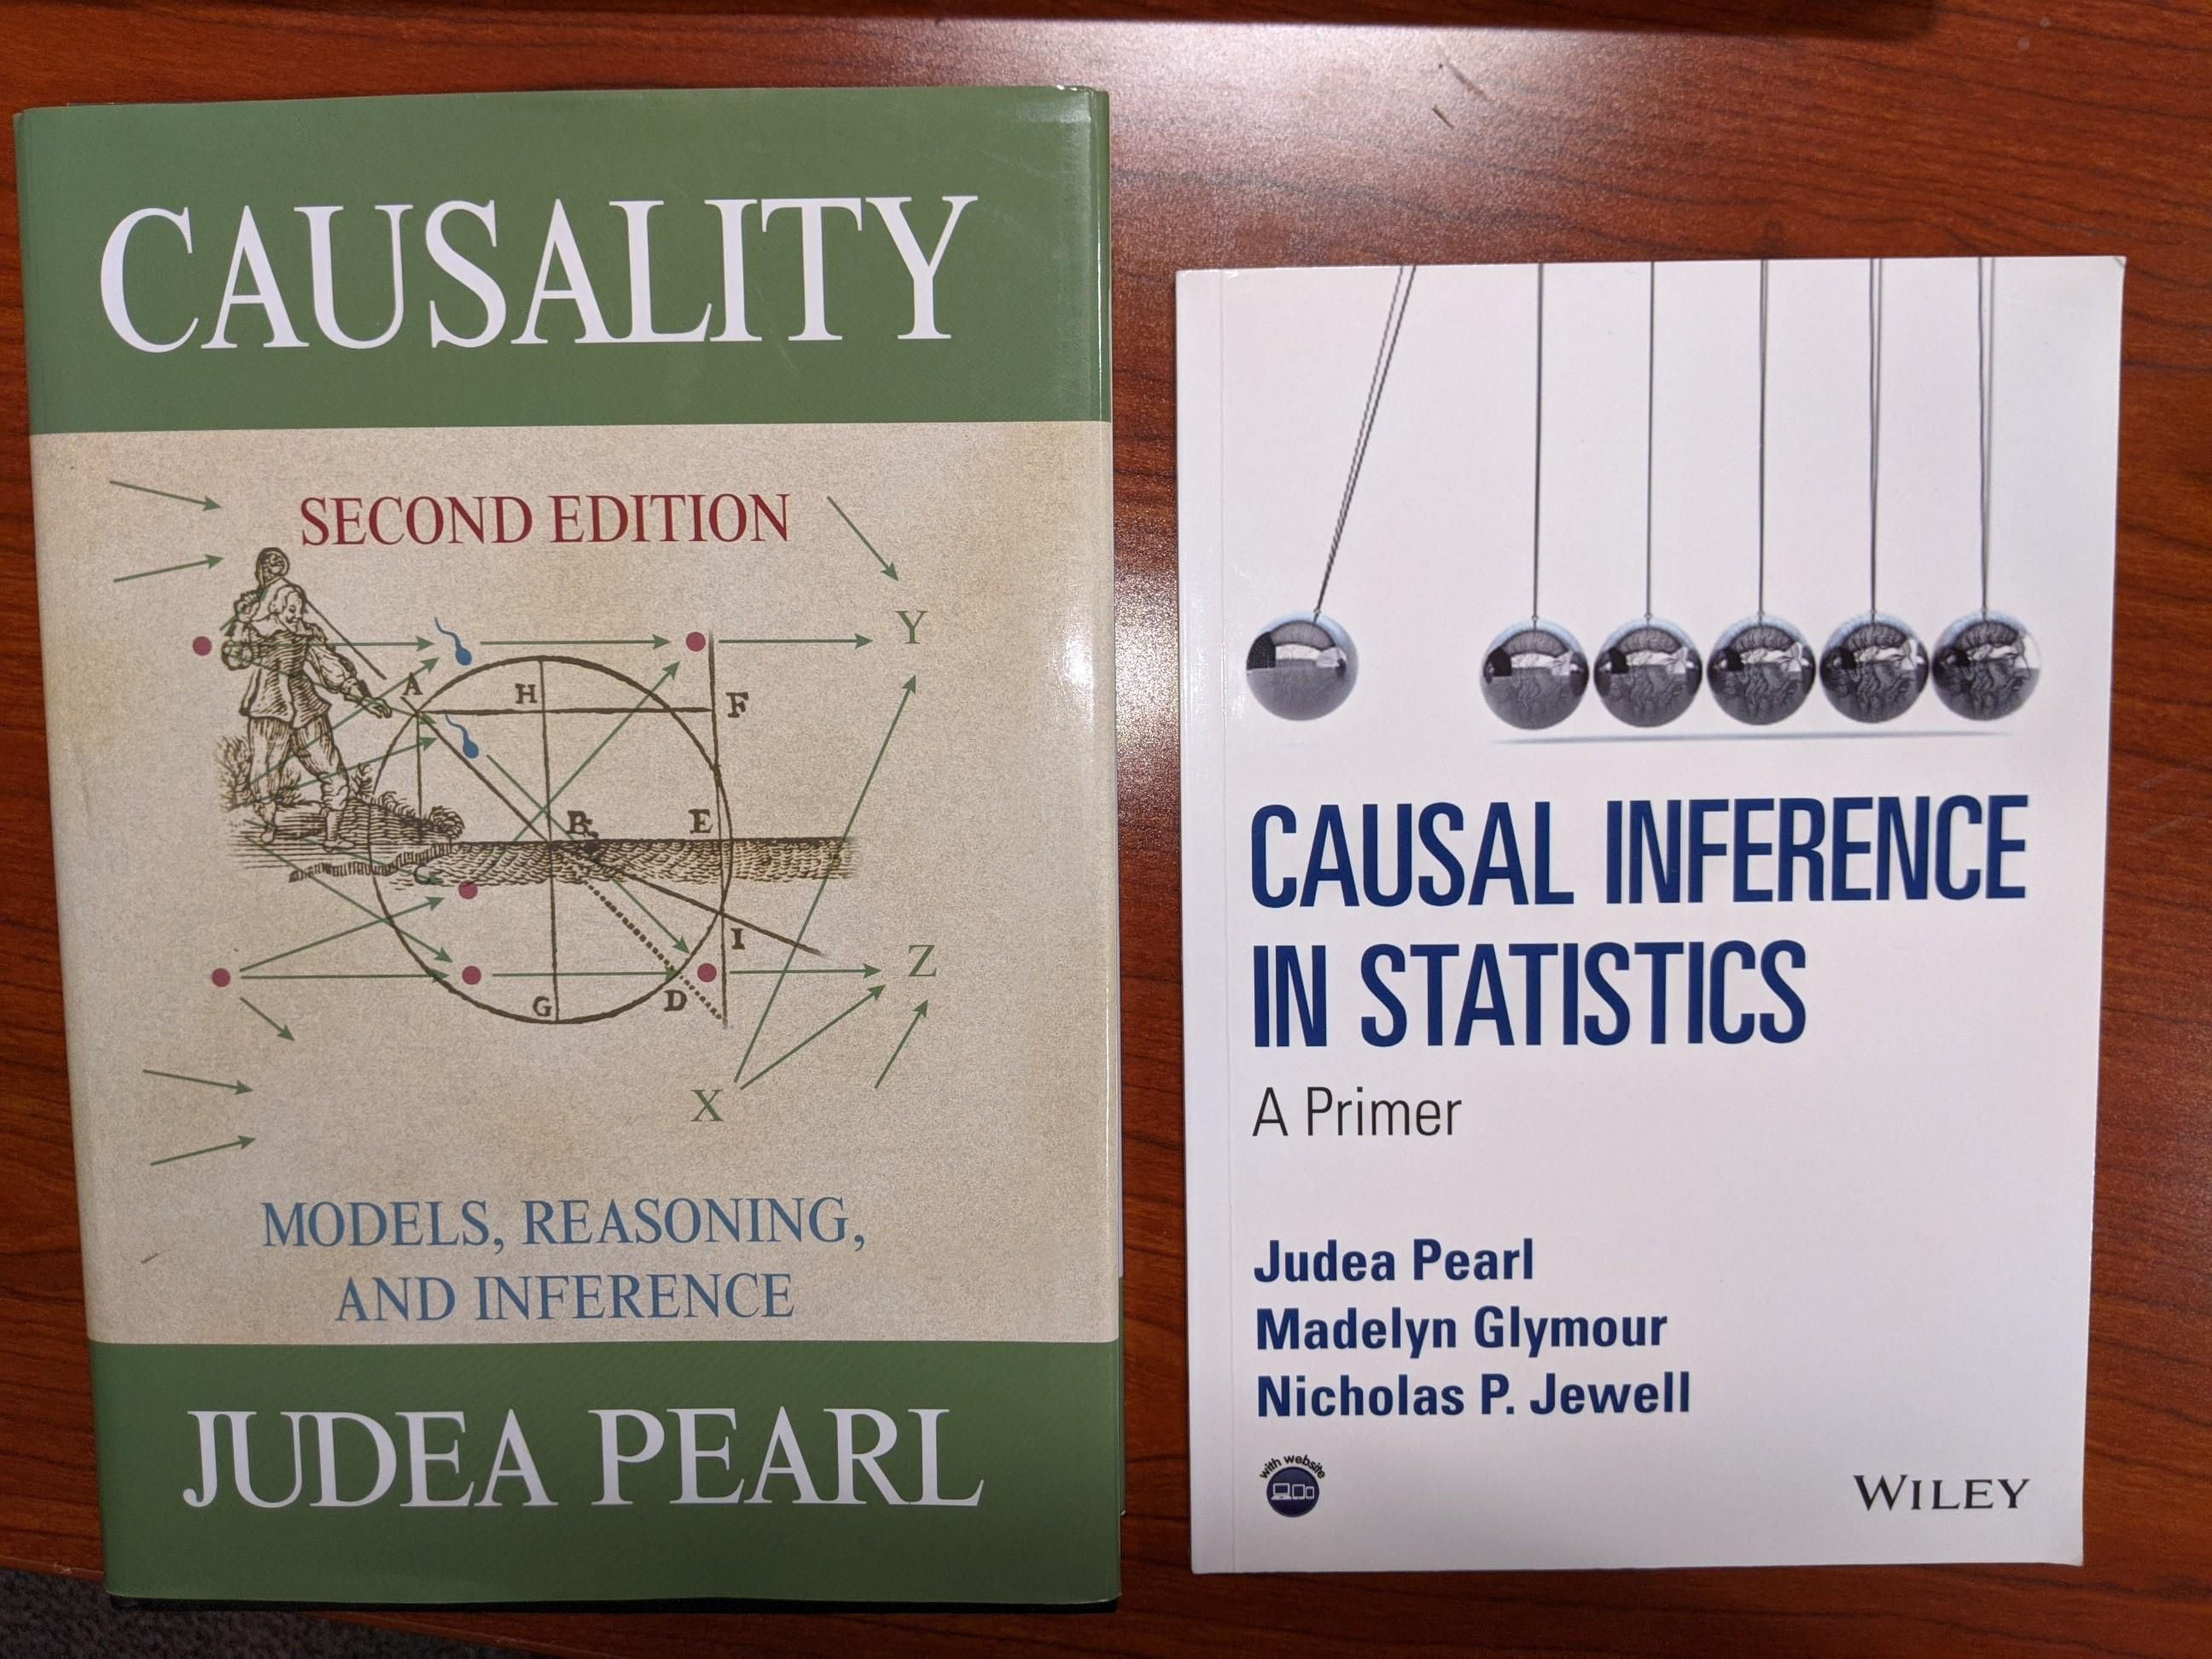
\includegraphics[width=0.7\textwidth]{pearl} \\
\end{frame}



\begin{frame}
  \frametitle{Example 3: Effect of effluent from a new power plant on
    fish species richness in a river}
  A new power plant is to be established along the Oconee River.  We
  know for several years beforehand that the plant will be built.  So
  a survey is designed where fish are sampled periodically above
  (upriver from) and below (downriver from) the site, with repeated
  surveys done before and after the plant goes on line.  These are
  then compared to assess the effect of the plant on species richness.   
\end{frame}


\begin{frame}
  \frametitle{Example 3: Effect of effluent from a new power plant on
    fish species richness in a river}
  \centering
  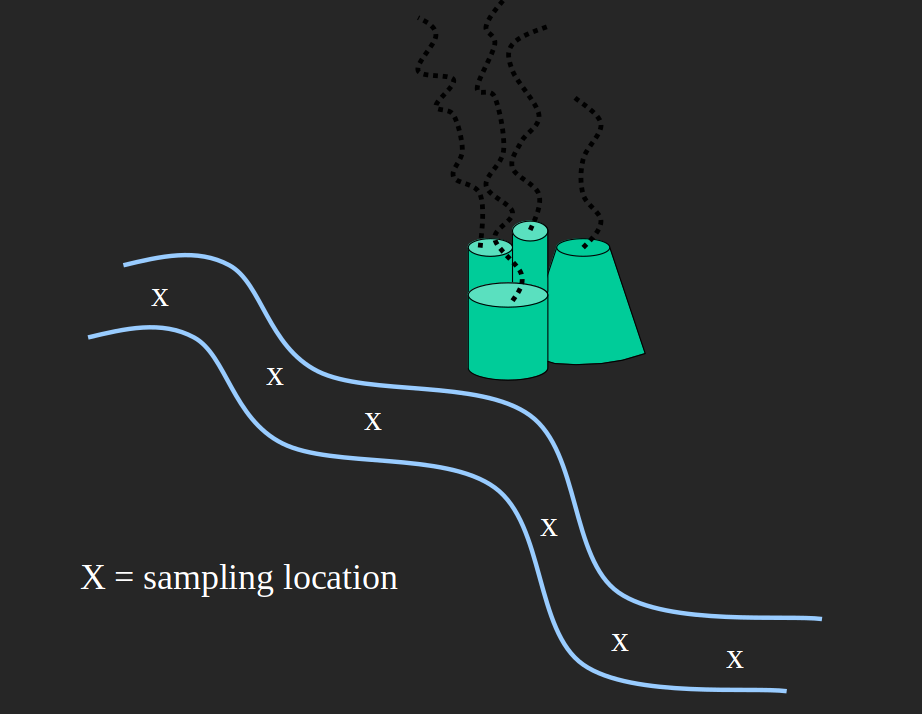
\includegraphics[width=0.9\textwidth]{power-plant-river} \\
\end{frame}


\begin{frame}
  \frametitle{Example 3: Effect of effluent from a new power plant on
    fish species richness in a river}
  \centering
  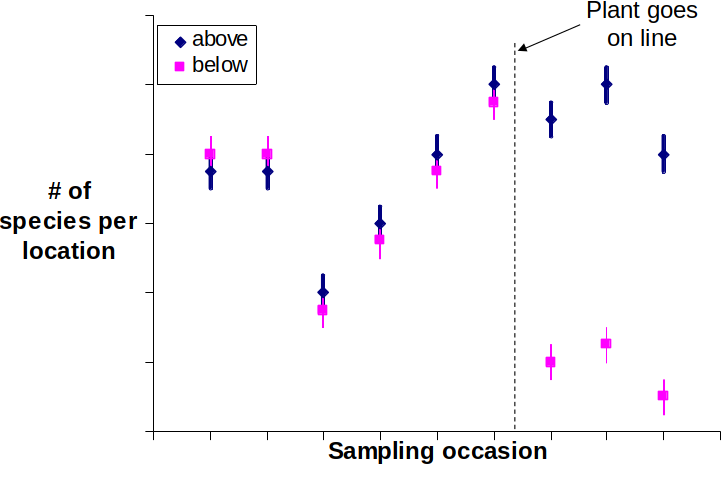
\includegraphics[width=0.8\textwidth]{power-plant} \\
\end{frame}




\begin{frame}
  \frametitle{Observational vs experimental research}
  Are manipulative experiments better than observation studies? \\
  \begin{itemize}
    \item Typically, yes, if good experimental design is used and the
      variables of interest can be manipulated.
    \item However, a poorly designed experiment can be worse than a good
      observational study and manipulative experiments aren't always
      possible. 
  \end{itemize}
  % \pause
  % \vfill
  % Consider using a combination of experimental and observational
  % methods.
\end{frame}


\begin{frame}
  \frametitle{Conclusions}
  What does this mean for graduate student research?
  \begin{itemize}[<+->]
    \item Graduate students only have a couple of years to create an
      interesting question, design a study to address that question,
      collect and analyze data, and write a thesis.
    \item Long-term study usually out of the question.
    \item Focus on a particular question in a broader framework.
    \item Often, students are handed a thesis topic. Pros and cons.
    \item Well-designed manipulative experiments usually make for
      stronger inference but are not always appropriate or possible. 
    \item Observational studies are fine, but there are many pitfalls
      to be wary of, e.g. confounders.
    \item Consider using a combination of observational and
      experimental methods.
  \end{itemize}
\end{frame}


\end{document}
